\subsection{Performance of the Filter}
The performance of the Kalman filter is tested through simulations. These are performed by applying some arbitrary inputs to the nonlinear model of the system derived in \autoref{chap:model}. The signals obtained are transformed into measurements by adding noise whose variance are those present in the physical sensors, as seen in \autoref{app:IMUVariances}.

In \autoref{fig:sim_yaw} the estimation of the heading, $\psi$, can be seen.
\begin{figure}[H]
    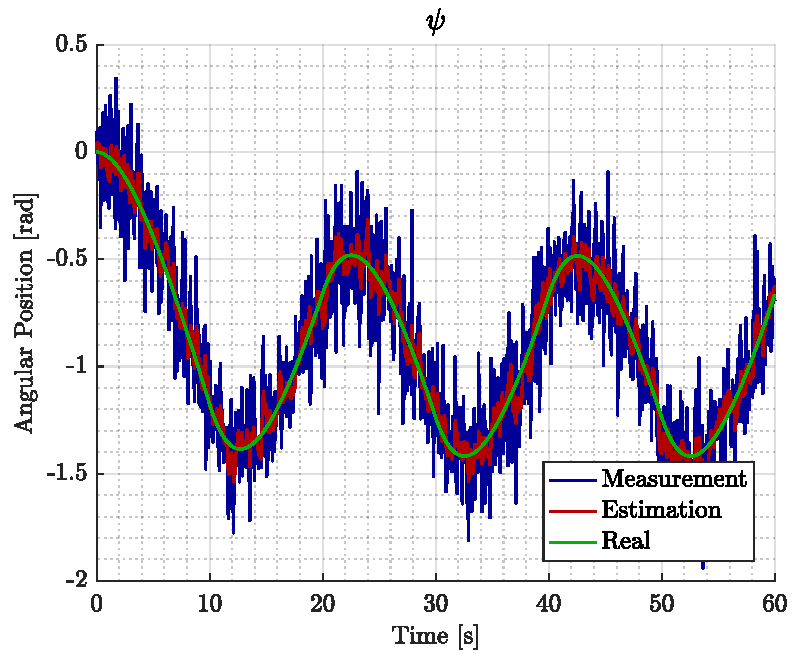
\includegraphics[width=0.5\textwidth]{figures/sim_yaw}
    \caption{Result of the estimation of the heading, compared to the real value in the simulation and the measurements.}
    \label{fig:sim_yaw}
\end{figure}

The filter is able to remove part of the noise present in the measurements, and gives a better results than the raw measurements.
%
The estimation of the angular velocity and acceleration around $z_\mathrm{b}$ can be seen in \autoref{fig:sim_yawdot} and \ref{fig:sim_yawddot}, respectively. The filter is able to give a correct estimate of the real signals even when there is no measurement, as it is the case for $\ddot{\psi}$.
%
\begin{figure}[H]
    \captionbox 
    {   
        Result of the estimation of the angular velocity around $z_\mathrm{b}$, compared to the real value in the simulation and the measurements.
        \label{fig:sim_yawdot}
    }                                                                 
    {                                                                  
        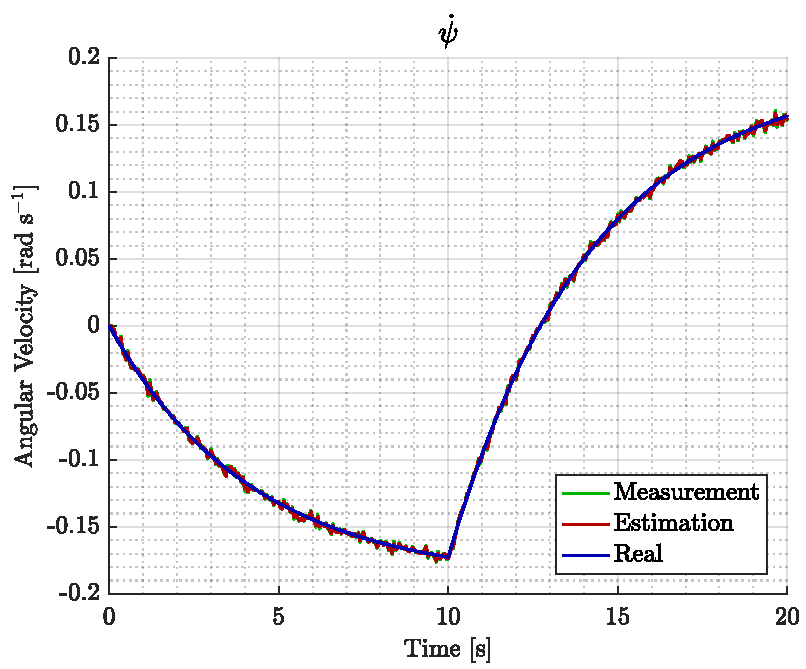
\includegraphics[width=.45\textwidth]{figures/sim_yawdot}         
    }                                                                    
    \hspace{5pt}                                                          
    \captionbox  
    {      
        Estimation of the angular acceleration around $z_\mathrm{b}$, compared to the real value.
        \label{fig:sim_yawddot}
    }                                                                          
    {
        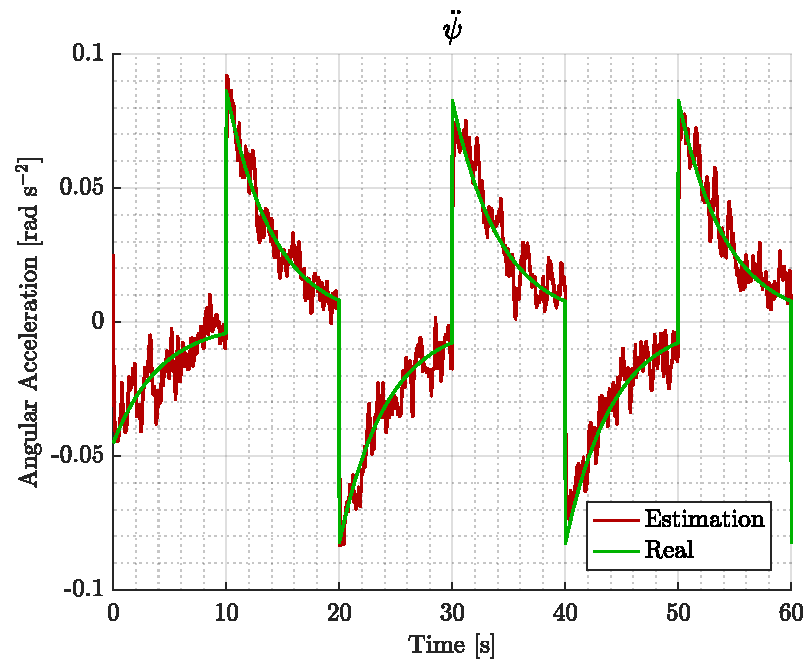
\includegraphics[width=.45\textwidth]{figures/sim_yawddot}
    }
\end{figure}
%
%\begin{figure}[H]
%    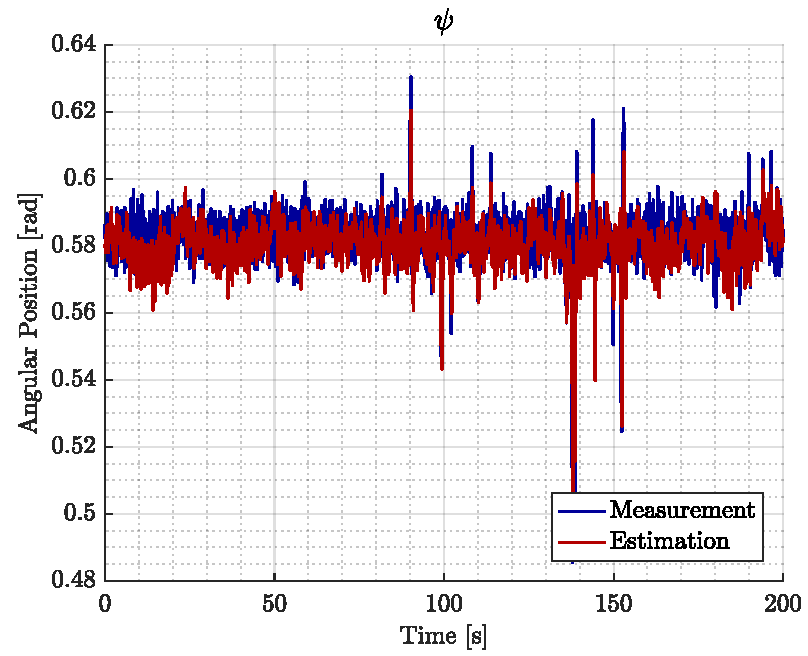
\includegraphics[width=0.5\textwidth]{figures/real_yaw}
%    \caption{}
%    \label{fig:real_yaw}
%\end{figure}
%
%\begin{figure}[H]
%    \captionbox 
%    {   
%        Result of the estimation of the angular velocity around $z_\mathrm{b}$, compared to the measurements.
%        \label{fig:real_yawdot}
%    }                                                                 
%    {                                                                  
%        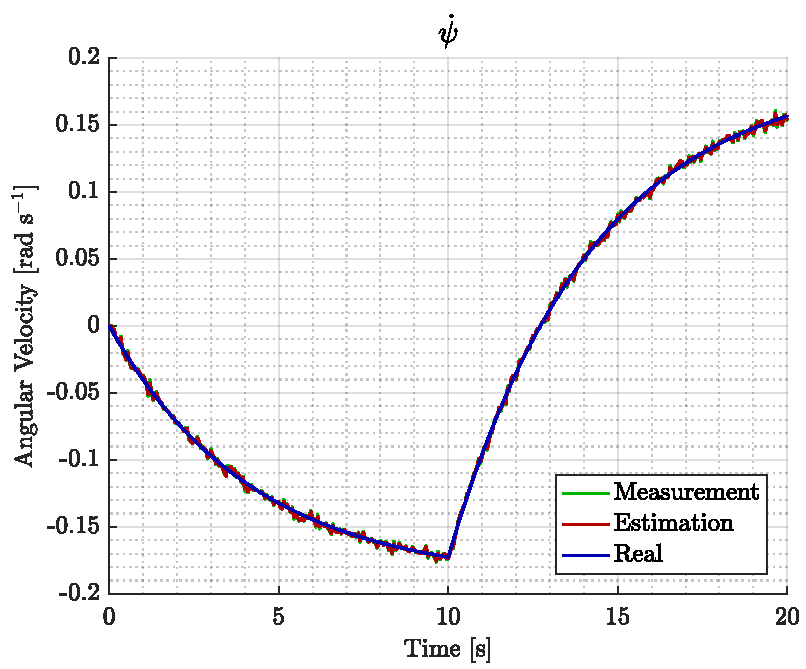
\includegraphics[width=.45\textwidth]{figures/sim_yawdot}         
%    }                                                                    
%    \hspace{5pt}                                                          
%    \captionbox  
%    {      
%        Estimation of the angular acceleration around $z_\mathrm{b}$.
%        \label{fig:real_yawddot}
%    }                                                                          
%    {
%        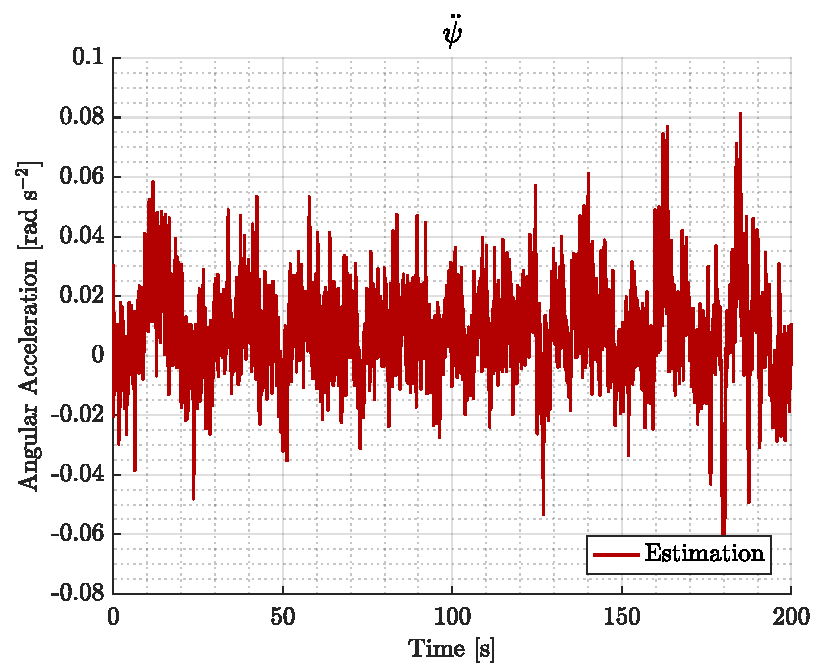
\includegraphics[width=.45\textwidth]{figures/real_yawddot}
%    }
%\end{figure}
%
%\cite{MSalari}